% Chapter 7: Sprint 4 - Approval Workflow & Status Management

\chapter{Sprint 4: Approval Workflow and Status Management}

\section{Introduction}

Sprint 4 implements the critical approval workflow that enables supervisors to review, validate, and approve completed interventions. This sprint introduces status tracking, audit trails, and notification mechanisms that provide transparency and control over the intervention lifecycle. The implementation ensures accountability and enables supervisors to manage quality assurance for all completed work.

The approval workflow integrates with the notification system to keep all stakeholders informed of intervention status changes, enabling efficient communication and timely decision-making throughout the organization.

\section{Sprint Preview and Objectives}

\subsection{User Stories}

\begin{enumerate}
\item \textbf{US-S4-001: Approval Workflow}
  \begin{itemize}
  \item \textbf{As a} supervisor
  \item \textbf{I want} to review and approve or reject completed interventions
  \item \textbf{So that} I ensure quality and control work delivery
  \item \textbf{Story Points:} 13
  \end{itemize}

\item \textbf{US-S4-002: Status History Tracking}
  \begin{itemize}
  \item \textbf{As a} coordinator
  \item \textbf{I want} to track status changes and reasons throughout intervention lifecycle
  \item \textbf{So that} I have complete audit trail of all modifications
  \item \textbf{Story Points:} 8
  \end{itemize}

\item \textbf{US-S4-003: Rejection with Feedback}
  \begin{itemize}
  \item \textbf{As a} supervisor
  \item \textbf{I want} to reject interventions with detailed feedback
  \item \textbf{So that} technicians understand required corrections
  \item \textbf{Story Points:} 8
  \end{itemize}

\item \textbf{US-S4-004: Status Notifications}
  \begin{itemize}
  \item \textbf{As a} system
  \item \textbf{I want} to notify stakeholders of status changes
  \item \textbf{So that} everyone is informed of intervention progress
  \item \textbf{Story Points:} 8
  \end{itemize}

\item \textbf{US-S4-005: Supervisor Dashboard}
  \begin{itemize}
  \item \textbf{As a} supervisor
  \item \textbf{I want} to view pending interventions awaiting approval
  \item \textbf{So that} I can quickly identify and process them
  \item \textbf{Story Points:} 8
  \end{itemize}
\end{enumerate}

\subsection{Sprint Goals}

\begin{enumerate}
\item \textbf{Approval Workflow:} Implement complete approval process with state transitions
\item \textbf{Status Management:} Track all status changes with audit trail
\item \textbf{Quality Assurance:} Enable supervisors to validate work and provide feedback
\item \textbf{Notifications:} Keep all stakeholders informed of status updates
\end{enumerate}

\section{Sprint Backlog}

The 45-point sprint focuses on workflow and status management:

\begin{table}[H]
\centering
\caption{Sprint 4 Backlog}
\label{tab:sprint4_backlog}
\begin{tabularx}{\textwidth}{|l|X|l|l|}
\hline
\textbf{ID} & \textbf{User Story} & \textbf{Points} & \textbf{Status} \\
\hline
S4-1 & Approval workflow & 13 & Completed \\
\hline
S4-2 & Status history tracking & 8 & Completed \\
\hline
S4-3 & Rejection with feedback & 8 & Completed \\
\hline
S4-4 & Status notifications & 8 & Completed \\
\hline
S4-5 & Supervisor dashboard & 8 & Completed \\
\hline
\textbf{Total} & & \textbf{45} & \\
\hline
\end{tabularx}
\end{table}

\section{Functional Specification}

\subsection{Intervention Status Lifecycle}

The intervention lifecycle includes the following statuses with specific transitions:

\begin{figure}[H]
\centering
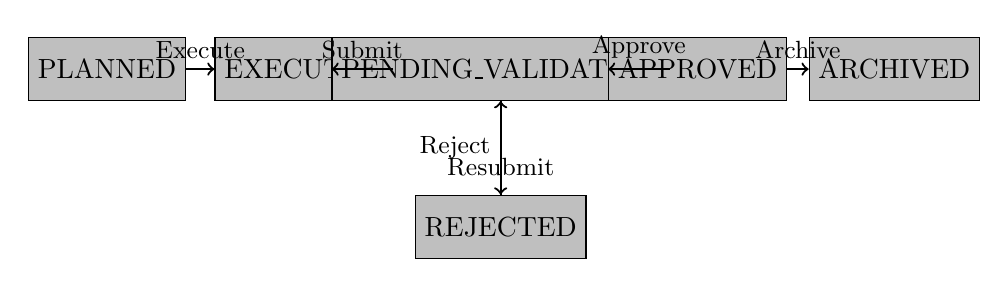
\begin{tikzpicture}[
    state/.style={rectangle, draw=black, fill=lightgray, minimum width=2cm, minimum height=0.8cm},
    arrow/.style={->, thick}
  ]
  
  \node[state] (planned) at (0, 0) {PLANNED};
  \node[state] (executed) at (2.5, 0) {EXECUTED};
  \node[state] (pending) at (5, 0) {PENDING\_VALIDATION};
  \node[state] (approved) at (7.5, 0) {APPROVED};
  \node[state] (archived) at (10, 0) {ARCHIVED};
  \node[state] (rejected) at (5, -2) {REJECTED};

  \draw[arrow] (planned) -- node[above, font=\small] {Execute} (executed);
  \draw[arrow] (executed) -- node[above, font=\small] {Submit} (pending);
  \draw[arrow] (pending) -- node[above, font=\small] {Approve} (approved);
  \draw[arrow] (approved) -- node[above, font=\small] {Archive} (archived);
  \draw[arrow] (pending) -- node[left, font=\small] {Reject} (rejected);
  \draw[arrow] (rejected) -- node[below, font=\small] {Resubmit} (pending);
  
\end{tikzpicture}
\caption{Intervention Status Lifecycle}
\label{fig:sprint4_lifecycle}
\end{figure}

\section{Conception}

\subsection{Class Diagram}

\begin{figure}[H]
\centering
\begin{tikzpicture}[node distance=2cm, auto]
  \node[umlclass] (request) at (0, 2) {
    RapportRequest\\
    --------------------\\
    - id: Long\\
    - status: Status\\
    - statusHistory: Set<StatusHistory>
  };

  \node[umlclass] (status) at (3, 2) {
    StatusHistory\\
    --------------------\\
    - id: Long\\
    - previousStatus: Status\\
    - newStatus: Status\\
    - changedAt: ZonedDateTime\\
    - changedBy: User
  };

  \node[umlclass] (reject) at (3, -1) {
    Reject\\
    --------------------\\
    - id: Long\\
    - reason: String\\
    - feedback: String\\
    - rejectedAt: ZonedDateTime
  };

  \node[umlclass] (user) at (7, 2) {
    User\\
    --------------------\\
    - id: Long\\
    - login: String\\
    - role: Role
  };

  \draw[->] (request) -- (status) node[midway, above] {has};
  \draw[->] (status) -- (user) node[midway, above] {trackedBy};
  \draw[->] (request) -- (reject) node[midway, right] {may have};

\end{tikzpicture}
\caption{Sprint 4 Class Diagram - Approval Workflow}
\label{fig:sprint4_class}
\end{figure}

\section{Realization}

\subsection{Backend Implementation}

\textbf{Status Enumeration:}
\begin{lstlisting}
public enum RapportStatus {
    PLANNED("Planifie"),
    EXECUTED("Excute"),
    PENDING_VALIDATION("En attente de validation"),
    APPROVED("Approuve"),
    REJECTED("Rejete"),
    ARCHIVED("Archive");

    private final String label;

    RapportStatus(String label) {
        this.label = label;
    }
}
\end{lstlisting}

\textbf{StatusHistory Entity:}
\begin{lstlisting}
@Entity
@Table(name = "status_history")
public class StatusHistory extends AbstractAuditingEntity {

    @Id
    @GeneratedValue(strategy = GenerationType.SEQUENCE)
    private Long id;

    @Enumerated(EnumType.STRING)
    private RapportStatus previousStatus;

    @Enumerated(EnumType.STRING)
    private RapportStatus newStatus;

    @Column(name = "changed_at")
    private ZonedDateTime changedAt;

    @ManyToOne
    private User changedBy;

    @ManyToOne
    private RapportRequest rapportRequest;
}
\end{lstlisting}

\textbf{Rejection Entity:}
\begin{lstlisting}
@Entity
@Table(name = "rejection")
public class Rejection {

    @Id
    @GeneratedValue(strategy = GenerationType.SEQUENCE)
    private Long id;

    @Column(name = "reason")
    private String reason;

    @Column(name = "feedback", columnDefinition = "TEXT")
    private String feedback;

    @Column(name = "rejected_at")
    private ZonedDateTime rejectedAt;

    @ManyToOne
    private User rejectedBy;

    @OneToOne
    private RapportRequest rapportRequest;
}
\end{lstlisting}

\textbf{Approval Service:}
\begin{lstlisting}
@Service
@Transactional
public class ApprovalService {

    private final RapportRequestRepository requestRepository;
    private final StatusHistoryRepository historyRepository;
    private final RejectionRepository rejectionRepository;
    private final NotificationService notificationService;
    private final CurrentUserService currentUser;

    public RapportRequestDTO approveIntervention(Long requestId) {
        RapportRequest request = requestRepository.findById(requestId)
            .orElseThrow();

        if (request.getStatus() != RapportStatus.PENDING_VALIDATION) {
            throw new InvalidStatusTransitionException();
        }

        // Record status change
        StatusHistory history = new StatusHistory();
        history.setPreviousStatus(request.getStatus());
        history.setNewStatus(RapportStatus.APPROVED);
        history.setChangedAt(ZonedDateTime.now());
        history.setChangedBy(currentUser.getCurrentUser());
        history.setRapportRequest(request);
        historyRepository.save(history);

        // Update request
        request.setStatus(RapportStatus.APPROVED);
        request = requestRepository.save(request);

        // Send notification
        notificationService.notifyApproval(request);

        return mapper.toDto(request);
    }

    public RapportRequestDTO rejectIntervention(
        Long requestId,
        String reason,
        String feedback) {

        RapportRequest request = requestRepository.findById(requestId)
            .orElseThrow();

        if (request.getStatus() != RapportStatus.PENDING_VALIDATION) {
            throw new InvalidStatusTransitionException();
        }

        // Create rejection record
        Rejection rejection = new Rejection();
        rejection.setReason(reason);
        rejection.setFeedback(feedback);
        rejection.setRejectedAt(ZonedDateTime.now());
        rejection.setRejectedBy(currentUser.getCurrentUser());
        rejection.setRapportRequest(request);
        rejectionRepository.save(rejection);

        // Update status
        StatusHistory history = new StatusHistory();
        history.setPreviousStatus(request.getStatus());
        history.setNewStatus(RapportStatus.REJECTED);
        history.setChangedAt(ZonedDateTime.now());
        history.setChangedBy(currentUser.getCurrentUser());
        history.setRapportRequest(request);
        historyRepository.save(history);

        request.setStatus(RapportStatus.REJECTED);
        request = requestRepository.save(request);

        // Notify technician of rejection
        notificationService.notifyRejection(request, feedback);

        return mapper.toDto(request);
    }
}
\end{lstlisting}

\textbf{REST Controller:}
\begin{lstlisting}
@RestController
@RequestMapping("/api/rapport-requests")
public class ApprovalController {

    private final ApprovalService approvalService;

    @PostMapping("/{id}/approve")
    @PreAuthorize("hasRole('SUPERVISOR')")
    public ResponseEntity<RapportRequestDTO> approve(@PathVariable Long id) {
        return ResponseEntity.ok(approvalService.approveIntervention(id));
    }

    @PostMapping("/{id}/reject")
    @PreAuthorize("hasRole('SUPERVISOR')")
    public ResponseEntity<RapportRequestDTO> reject(
        @PathVariable Long id,
        @RequestBody RejectionDTO rejectionDTO) {

        return ResponseEntity.ok(approvalService.rejectIntervention(
            id,
            rejectionDTO.getReason(),
            rejectionDTO.getFeedback()
        ));
    }

    @GetMapping("/pending")
    @PreAuthorize("hasRole('SUPERVISOR')")
    public ResponseEntity<Page<RapportRequestDTO>> getPendingRequests(
        @PageableDefault(size = 20) Pageable pageable) {

        Page<RapportRequest> pending = requestRepository.findByStatus(
            RapportStatus.PENDING_VALIDATION,
            pageable);

        return ResponseEntity.ok(pending.map(mapper::toDto));
    }

    @GetMapping("/{id}/history")
    public ResponseEntity<List<StatusHistoryDTO>> getStatusHistory(@PathVariable Long id) {
        List<StatusHistory> history = historyRepository.findByRapportRequestId(id);
        return ResponseEntity.ok(history.stream()
            .map(mapper::toDto)
            .collect(Collectors.toList()));
    }
}
\end{lstlisting}

\subsection{Frontend Implementation}

\textbf{Approval Component:}
\begin{lstlisting}
@Component({
  selector: 'app-approval',
  templateUrl: './approval.component.html',
  styleUrls: ['./approval.component.css']
})
export class ApprovalComponent implements OnInit {
  pendingInterventions: RapportRequest[] = [];
  selectedIntervention: RapportRequest | null = null;
  rejectionForm: FormGroup;
  isLoading = false;

  constructor(
    private rapportService: RapportRequestService,
    private formBuilder: FormBuilder,
    private notificationService: NotificationService
  ) {
    this.rejectionForm = this.formBuilder.group({
      reason: ['', Validators.required],
      feedback: ['', Validators.required]
    });
  }

  ngOnInit(): void {
    this.loadPendingInterventions();
  }

  loadPendingInterventions(): void {
    this.isLoading = true;
    this.rapportService.getPendingApprovals()
      .subscribe({
        next: (data) => {
          this.pendingInterventions = data;
          this.isLoading = false;
        },
        error: () => this.isLoading = false
      });
  }

  approve(intervention: RapportRequest): void {
    if (!confirm('Are you sure you want to approve this intervention?')) {
      return;
    }

    this.rapportService.approveIntervention(intervention.id)
      .subscribe({
        next: () => {
          this.notificationService.showSuccess(
            'Intervention approved successfully');
          this.loadPendingInterventions();
        },
        error: (error) => {
          this.notificationService.showError(
            'Failed to approve intervention');
        }
      });
  }

  reject(intervention: RapportRequest): void {
    if (this.rejectionForm.invalid) {
      return;
    }

    this.rapportService.rejectIntervention(
      intervention.id,
      this.rejectionForm.value)
      .subscribe({
        next: () => {
          this.notificationService.showSuccess(
            'Intervention rejected');
          this.rejectionForm.reset();
          this.loadPendingInterventions();
        },
        error: () => {
          this.notificationService.showError(
            'Failed to reject intervention');
        }
      });
  }

  viewHistory(intervention: RapportRequest): void {
    this.rapportService.getStatusHistory(intervention.id)
      .subscribe((history) => {
        // Display status history dialog
      });
  }
}
\end{lstlisting}

\section{Tests and Validation}

\subsubsection{Approval Workflow Tests}

\begin{lstlisting}
@SpringBootTest
class ApprovalServiceTest {

    @Autowired
    private ApprovalService approvalService;

    @MockBean
    private NotificationService notificationService;

    @Test
    void approveIntervention() {
        RapportRequest request = createPendingIntervention();

        RapportRequestDTO result = approvalService
            .approveIntervention(request.getId());

        assertThat(result.getStatus()).isEqualTo(RapportStatus.APPROVED);
        verify(notificationService).notifyApproval(any());
    }

    @Test
    void rejectIntervention() {
        RapportRequest request = createPendingIntervention();

        RapportRequestDTO result = approvalService.rejectIntervention(
            request.getId(),
            "Missing information",
            "Please provide additional photos");

        assertThat(result.getStatus()).isEqualTo(RapportStatus.REJECTED);
        verify(notificationService).notifyRejection(any(), anyString());
    }

    @Test
    void validateStatusTransitions() {
        RapportRequest request = createArchivedIntervention();

        assertThatThrownBy(() -> 
            approvalService.approveIntervention(request.getId()))
            .isInstanceOf(InvalidStatusTransitionException.class);
    }
}
\end{lstlisting}

\section{Conclusion}

Sprint 4 successfully implemented the approval workflow and comprehensive status management system. Supervisors now have complete visibility and control over the intervention lifecycle, with detailed audit trails tracking all status changes. The rejection workflow enables constructive feedback and continuous improvement, while notifications ensure stakeholders remain informed of all changes.

Key achievements:
\begin{itemize}
\item Complete approval workflow with state transitions
\item Status history tracking for full audit trail
\item Rejection with detailed feedback mechanism
\item Real-time notifications for status changes
\item Supervisor dashboard for pending reviews
\end{itemize}

Sprint 5 will focus on advanced reporting capabilities and system optimization, enabling comprehensive analysis of intervention data and operational metrics.
